\chapter*{LỜI CAM ĐOAN}
\addcontentsline{toc}{chapter}{LỜI CAM ĐOAN}

Chúng tôi xin cam đoan rằng toàn bộ nội dung trong bản báo cáo Đồ án Chuyên ngành Công nghệ Thông tin 2 với đề tài \textbf{``Hệ thống Quản lý Ký túc xá Thông minh (SmartDorm)''} là công trình nghiên cứu và thực nghiệm độc lập do chính nhóm tác giả thực hiện dưới sự hướng dẫn khoa học của \textbf{TS. Phù Trần Tín}.

Các số liệu, mã nguồn chương trình, sơ đồ nguyên lý mạch phần cứng và kết quả thực nghiệm được trình bày trong báo cáo hoàn toàn trung thực, phản ánh chính xác kết quả xây dựng, đo đạc và kiểm thử hệ thống trong thực tế. Toàn bộ các tài liệu tham khảo, thư viện mã nguồn mở và công trình liên quan đều được trích dẫn đầy đủ, rõ ràng và tuân thủ nghiêm ngặt các quy định về quyền sở hữu trí tuệ.

Nếu phát hiện có bất kỳ sự gian lận nào, chúng tôi xin hoàn toàn chịu trách nhiệm về nội dung Đồ án của mình. Trường Đại học Tôn Đức Thắng không liên quan đến những vi phạm tác quyền, bản quyền do chúng tôi gây ra trong quá trình thực hiện (nếu có).

\vspace{1.5cm}
\noindent
\begin{minipage}[t]{0.48\textwidth}
    \centering
    \textit{TP. Hồ Chí Minh, năm 2026}\\[0.2cm]
    \textbf{Tác giả}\\[0.1cm]
    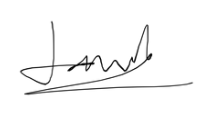
\includegraphics[height=1.8cm]{figures/signature_manh.png}\\[0.1cm]
    \textbf{Nguyễn Tấn Mạnh}\\[0.1cm]
    MSSV: 52300221
\end{minipage}
\hfill
\begin{minipage}[t]{0.48\textwidth}
    \centering
    \textit{TP. Hồ Chí Minh, năm 2026}\\[0.2cm]
    \textbf{Tác giả}\\[0.1cm]
    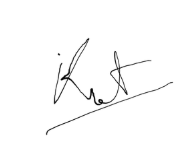
\includegraphics[height=1.8cm]{figures/signature_kiet.png}\\[0.1cm]
    \textbf{Võ Anh Kiệt}\\[0.1cm]
    MSSV: 523H0048
\end{minipage}
\newpage
